\chapter{Background and Related Work Analysis}\label{bg}
In this chapter we provide the reader with a review of the basic knowledge in fields of optimization problems and approaches for solving them.
A reader, experienced in field of Optimization and Search Problems, may consider this chapter as an obvious discussion of well-known facts. 
If such notions as \textit{Parameter Tuning} and \textit{Parameter Control} are not familiar to you or seems the same, we highly encourage you to spend some time reading this chapter carefully.
In any case, it is worth for everyone to refresh the knowledge with coarse-grained description of topics, mentioned in this section and examine the examples of hyper-heuristics in Section~\ref{bg: hh examples} and systems for parameter tuning in Section~\ref{bg: parameter tuning expamples}.

The structure of this Chapter is defined as follows. Firstly, we give an informal definition of optimization problem and enumerate possible solver types in Section~\ref{bg:section problems and solvers}. Secondly, we pay attention to the heuristic solvers, their weak points and No Free Lunch Theorem in Section~\ref{bg: section heuristics}. Afterwards, in Section~\ref{bg: section Parameters Setting} we discuss the influence of parameter setting and possible approaches to set the parameters. Section~\ref{bg: section cash}, dedicated to \emph{Combined Algorithm Selection and Hyper-parameter Tuning} problem, is followed by conclusion on the literature analysis outlining the thesis' scope in Section~\ref{bg: section conclusion}.

\section{Optimization Problems and their Solvers}\label{bg:section problems and solvers}
Our life is full of different difficult and sometimes contradicting choices. Optimization is an art of making good decisions.

A decision between working hard or going home earlier, to buy cheaper goods or to follow brands, to isolate ourselves or to visit friends during the quarantine, to spend more time for planning trip or to start it instantly. Each decision that we make, has its consequences.

Figure~\ref{bg:pic:Optimization tradeoff} outlines the trade-off between a decision quality and an amount of effort spent. The underlying idea of the research in optimization problems solving sphere is to squash this curve simultaneously down and to the left thus, deriving a better result with less cost when solving the optimization problem.

\svgpath{{graphics/Background/}}
\begin{figure}
	\centering
	\includesvg[width=0.7\textwidth]{optimization_concept}
	\caption{Optimization trade-off.}
	\label{bg:pic:Optimization tradeoff}
\end{figure}
\todoy{axes labels should be distinguishable from axes values (Dima review)}

\subsection{Optimization Problems}\label{BG: subsection OPs}
While the \emph{Search Problem} (SP) defines the process of finding a possible solution for the \emph{Computation Problem}, an \emph{Optimization Problem} (OP) is the special case of the SP, focused on the process of finding the \emph{best possible} solution for computation problem~\cite{goldreich2010p}.

In this thesis we focus on the optimization problems.

A lot of studies in this field have tried to formalize the concept of OP, but the underlying notion is so vast that it is hard to exclude the application domain from the definition. The description of every possible optimization problem and all approaches for solving it is out of this thesis scope, but a coarse-grained review should be presented in order to make sure that everyone reading this thesis is familiar with all used here terms and notions. 

First, let us define the optimization \emph{subject}. Analytically, it could be represented as the function $Y = f(X)$ that accepts some input $X$ and reacts on it, providing an output $Y$. Informally, it could be imagined as the Target System $f$ (TS), shown on Figure~\ref{bg:pic:Target System}. It accepts the input information with its \emph{inputs}} $X_n$ sometimes also called variables or parameters, processes them performing some \emph{Task} and produces the result on its \emph{outputs} $Y_m$.

\begin{figure}[!h]
	\centering
	\includesvg[width=0.5\textwidth]{TargetSystem}
	\caption{Optimization Target System.}
	\label{bg:pic:Target System}
\end{figure}

Each (unique) pair of sets $X_n^i$ and respective $Y_m^i$ form $Solution^i$ for computational problem.
All possible inputs $X^i$, where $i=1...N$ form a \emph{Search Space} of size $N$, while all outcomes $Y^i$, where $i=1...M$ form an \emph{Objective Space} of size $M$.

The solution characterized by the \emph{objective value(s)} — a quantitative measure of TS performance that we want to minimize or maximize in the optimization problems. We could obtain those value(s) directly, by reading the output on $Y_m$, or indirectly, for instance, noting the wall clock time TS took to produce the output $Y^i$ for given~$X^i$. The solution objective value(s) form an \emph{object} of Optimization. 
For the sake of simplicity we here use $Y_m$, \textit{outputs} or \textit{objectives} interchangeably as well as $X_n$, \textit{variables} or \textbf{parameters}.

\todoy{figure for classification}
Next, let us highlight the Target System characteristics. In works~\cite{biegler2004retrospective,figueira2014hybrid,deb2014multi,amaran2016simulation} dedicated to solving OPs, the authors distinguished OP characteristics that overlap through each of these works. Among them, we found those properties the most important:
\begin{itemize}[itemsep=8pt]
	\item \textbf{Input data type} of $X_m$ is a crucial characteristic. All input variables could be (1) \emph{discrete}, where representatives are binary strings, integer-ordered, or categorical data, (2) \emph{continuous}, where variables are usually a range of real numbers, or (3) \emph{mixed}, as the mixture of the previous two cases.

	\item \textbf{Constraints} describe the relationships among inputs and explain the dependencies in allowable values for them. As an example, imagine that having $X_n$ equal to $value$ implies that $X_{n + k}$ should not appear at all, or could take only some subset of all possible values.
	
	\item \textbf{Type of target system} is an amount of exposed knowledge about the dependencies $X \rightarrow Y$ before the optimization process starts. With respect to this, an Optimization could be: \emph{white box} — it is possible to derive the algebraic model of TS,\emph{Grey Box} — the amount of exposed knowledge is significant, but not enough to build the algebraic model and \emph{Black Box} — the exposed knowledge is mostly negligible.
	%In this case the Derivative Free Optimization approaches (such as Surrogate Optimization, different Meta-|Hybrid-|Hyper-Heuristics)  are applicable.
	% http://downloads.hindawi.com/journals/mpe/2015/647234.pdf

	%\paragraph{Dependency types} could be  The inputs to outputs dependencies the of Target System could also be distinguished form perspective of linearity \cite{biegler2004retrospective,figueira2014hybrid}.
	%\textit{Linear dependencies} reveal the Linear Programming Optimization approaches, while with \textbf{Nonlinear dependencies} one should consider Nonlinear Programming.

	\item \textbf{Determinism} of TS is one of possible challenges, when the output is uncertain. TS is \emph{deterministic}, when it each time provides an equal output for the same input. However, in most real-life challenges engineers tackle \emph{stochastic} systems, whose output is affected by random processes happened inside TS. 

	\item \textbf{Cost of evaluation} is an amount of resources (energy, time, money, etc.) TS should spend to produce the output for particular input. It varies from \emph{cheap}, when TS could be an algebraic formula and Task evaluation is a simple mathematic computation, to very expensive, when the TS is a pharmaceutical company, and the Task is to perform a whole bunch of tests for a new drug, which may last years. 

	\item \textbf{Number of objectives} is a size of output vector $Y_m^i$. With regard to this, the optimization could be either Single- ($m=1$), or Multi- ($m=2...M$) objective, where the result is either single solution, or a set of non-dominated (Pareto-optimal) solutions respectively.
\end{itemize}

Most optimization problem types could be obtained by combining different types of each characteristic listed above.

In this thesis we tackle practical combinatorial problems where the most prominent examples are Bin Packing~\cite{martello1990bin}, Job-shop Scheduling~\cite{blazewicz1996job} or Vehicle Routing~\cite{toth2002vehicle} Optimization Problems.
All combinatorial problems are \emph{NP-Complete} meaning they are in both \emph{NP} (solution is verifiable in polynomial time) and \emph{NP-Hard} (problem can be transformed to other NP-Complete problem in polynomial time, allowing using different solving algorithm) complexity classes\cite{garey1979computers}.

As an example, let's grasp these characteristics for Traveling Salesman Problem (TSP)~\cite{applegate2006traveling} — an instance of the Vehicle Routing Problem~\cite{laporte1992vehicle} and one of the most frequently studied combinatorial OP (here we consider deterministic and symmetric TSP).
The informal definition of TSP is as follows: ``Given a set of $N$ cities and the distances between each of them, what is the shortest path that visits each city once and returns to the origin city?''
With respect to our previous definition of the optimization problem, the target system here is a function that evaluates the length of proposed path. The TSP distance (or cost) matrix is used in this function for the evaluation and it is clear that this TS exposes all internal knowledge thus, it is a white box.
The input $X_n$ is a vector of city indexes thus, the type of input data is non-negative integers. There are two constraints for the path: it should contain only unique indexes (visit each city only once) and it should start and end from the same city:~$[2 \rightarrow 1 \rightarrow ... \rightarrow 2]$.
Since the cost matrix is fixed and not changing during the solving process, the TS is considered to be deterministic and cost for two identical paths are always the same (nevertheless, there exist Dynamic TSP where the cost matrix changes at runtime to reflect a more realistic real-time traffic updates\cite{cheong2011dynamic}).
It is cheap to compute a cost for a given path using the cost matrix thus, overall Solution evaluation in this OP is cheap, but the overall number of Solutions is $N!$. Since we are optimizing only the route distance, this is a single-objective OP.


\subsection{Optimization Problem Solvers}\label{BG: subsection OP Solvers}
Most Optimization Problems could be solved by an exhaustive search, though trying all possible combinations of input variables and choosing one providing the best objective value. This approach guarantees to find globally optimal solution to OP. But when the Search Space size significantly increases, the amount of time needed for brute-force search becomes infeasible and in many cases even relatively small problem instances could not be solved by an enumeration.

% TODO: highlight that exchaustive search provides guaranteed optimality

Here different optimization techniques come into play, and exposed by Target System characteristics could restrict and sometimes strictly define the applicable approach.
For instance, imagine you have white box deterministic TS with discrete constrained input data and cheap evaluation. The OP in this case could be solved using Integer Linear Programming, or heuristics approaches. If this TS turned out to be a black box, the ILP approaches will not be applicable anymore and one should consider using heuristics~\cite{biegler2004retrospective}.

Again, there exist a lot of different characteristics for Optimization Problem Solvers classification, but they are a subject of many surveying works for instance~\cite{biegler2004retrospective}. Here as the point of interest we decided to highlight only two of them.

\begin{itemize}[itemsep=8pt]
	\item \textbf{Final solution quality} perspective.
	\begin{enumerate}
		\item \textbf{Exact} Solvers are those algorithms that always provide an optimal Solution for OP.
		\item \textbf{Approximate} Solvers produce a sub-optimal output with guarantee in quality (some order of distance to the optimal solution).
		\item \textbf{Heuristics} Solvers do not give any worst-case guarantee for the final result quality.
	\end{enumerate}
	
	\item \textbf{Solution availability} perspective.
	\begin{enumerate}
		\item \textbf{Finalizing} algorithms, that report the results only at the end of their run.
		\item \textbf{Anytime} algorithms, designed for stepwise solution improvement, while solving the OP thus, could expose intermediate results.
	\end{enumerate}
	
\end{itemize}

Each of these algorithm characteristics provide their own advantages paying sacrificing other. As instance, if solution is not available at any time, one will not be able to control the optimization process, but if it does available, the overall performance may suffer. 
If the former features are more or less self-explanatory, we explain the later ones in more details including examples.

\subsubsection{Solution Quality Classes}
\paragraph{Exact Solvers.}
As stated previously, the exact algorithms are those, which always solve an OP to guaranteed optimality.

For some OP it is possible to develop an effective algorithm that is much faster than the exhaustive search — they run in super-polynomial time instead of exponential still providing an optimal solution. As authors claimed in~\cite{woeginger2003exact}, if the common belief $P \ne NP$ is true thus, super-polynomial time algorithms are the best we can hope to get when dealing with NP-complete (combinatorial) problems.

By the definition in~\cite{fomin2013exact}, the objective of an \textit{exact algorithm} is to perform much better (in terms of running time) than exhaustive search. In both works~\cite{woeginger2003exact,fomin2013exact} authors enumerated the main techniques for designing exact algorithms, each contributing in this `better' independently thus later they could be combined.

Here is a brief explanation of them:
\begin{itemize}[itemsep=8pt]
	\item \textbf{Branching and bounding} techniques when applied to original problem, split the search space of all possible solutions (e.g. exhaustive enumeration) to set of smaller sub-spaces. More formally this process called \textit{branching the search tree} into sub-trees. This is done with an intent to prove that some sub-spaces never lead to an optimal solution and thus could be rejected.
	
	\item \textbf{Dynamic programming across the sub-sets} techniques in some sort could be combined with the mentioned above branching techniques. After forming sub-trees, the dynamic programming attempts to derive solutions for smaller subsets and later combine them into solutions for lager subsets unless finally original search space solution obtained.
	
	\item \textbf{Problem preprocessing} could be applied as an initial phase of the solving process. This technique is dependable upon the underlying OP, but when applied properly, significantly reduces the running time. A toy example from~\cite{woeginger2003exact} elegantly illustrate this technique: imagine problem of finding a pair of two integers $x_i$ and $y_i$ that sum up to integer $S$ in $X_k$ and $Y_k$ sets of unique numbers ($k$ here denotes the size of sets). The exhaustive search will enumerate all $x-y$ pairs in $O(k^2)$ time. But one could first preprocess the data sorting it, after that use bisection search repeatedly in this sorted array and search for $k$ values $S - y_i$. The overall time complexity reduces to $O(k\log(k))$.
\end{itemize}

\paragraph{Approximate Solvers.} When the OP cannot be solved to optimal in polynomial time, people start thinking in alternative ways to tackle it and commonly decide to relax their requirements to optimization.
Approximate algorithms are representatives of the theoretical computer science field that have been created in order to tackle the \textit{computationally difficult white box OP} (not solvable in super-polynomial time). Words of Garey and Johnson (computer scientists, authors of \textit{Computers and intractability} book~\cite{garey1979computers}) could play a perfect description of such approaches, built on mathematical proofs: ``I can't find an efficient algorithm, but neither can all of these famous people.''
%If the widely believed conjecture $P \ne NP$ is true, a wide range of OPs (ILP) are $NP-hard$ and cannot be solved with exact solvers in polynomial time, thus require relaxation either in efficiency or quality of optimization.

In contradistinction to exact, approximate algorithms relax the quality requirements and solve an OP effectively with the provable assurances on the result distance from an optimal solution~\cite{williamson2011design}. The worst-case results quality guarantee is crucial in design of approximation algorithms and also involves mathematical proofs. 

One may ask a reasonable question ``How do these algorithms guarantee on quality, if the optimal solution is unknown ahead?'' Certainly it sounds contradicting, since knowing the optimal solution cancels an optimization problem itself. The answer to this question highlights a key technique in the design of approximation algorithms that is out of this thesis scope.

In~\cite{williamson2011design} authors provided several techniques of an approximate solvers design. For instance, the \textbf{Linear Programming} relaxation plays a central role in approximate solvers. It is well known that solving the ILP is \textit{NP-hard} problem, however it could be relaxed to polynomial-time solvable Linear Programming. %Those, one of techniques is relaxation of ILP to LP. An optimal solution for LP will have value $S_LP \le S_IP = OPT$ (for the minimization case). Here we could derive a lower bound for the original minimization or upper bound for maximization problem. 
Later fractional solution for the LP will be rounded to obtain a feasible solution for the ILP % that is within a cerain factor $f$ the value of the LP $S_LP$. Thus, the ILP solution will cost no more than $f * OPT$.
and different rounding strategies define separate technique for approximate solvers~\cite{williamson2011design}: 
\begin{itemize}[itemsep=8pt]
	\item \textbf{Deterministic rounding} follows predefined ahead strategy, while
	\item \textbf{Randomized rounding} will perform a round-up of each fractional solution value to integer uniformly.
\end{itemize}

In contrast to rounding, another technique requires building a \textit{Dual Linear Program} (DLP) for given Linear Program. This approach utilizes a \textit{weak} and \textit{strong duality} properties of DLP to derive the distance of LP solution to an optimal solution of original ILP. Other properties of DLP form a basis for \textbf{Primal-dual} algorithms. They start with a dual feasible solution and use dual information to derive a solution (possibly infeasible) for primal linear program. If the \textit{primal} solution is infeasible, algorithm modifies dual solution to increase the values of the dual objective function. In any case, these approaches are far beyond thesis scope, but in case of interest, reader could start own investigation from~\cite{williamson2011design}. 


\paragraph{Heuristics.} In contradiction to mentioned above solvers, heuristics do not provide any guarantee on the Solution quality. They are applicable not only to white box TS, but also to black box cases. These approaches are sufficient to quickly reach immediate, short-term goal in cases, where finding an optimal solution is impossible or impractical because of the huge search space size.

As in previous approaches, here exist many facets for classification.
We will start from the largest one, namely \textit{level of generality}:
\begin{itemize}[itemsep=8pt]
	\item \textbf{Simple heuristics} are algorithms, specifically designed to tackle concrete problem. They fully rely on the domain knowledge, obtained from Optimization Problem. Simple heuristics do not provide any mechanisms to escape a local optimum and thus could be easily trapped to it~\cite{pearl1984intelligent}.
	
	\item \textbf{Meta-heuristics} are high-level heuristics that not hardly rely on domain knowledge, but also provide some level of generality to control the search. Those, they could be applied to broader range of OPs. Often they are nature-inspired and comprise mechanisms to escape a local optima, but may converge slower than simple heuristics. For more detailed explanation we refer survey~\cite{bianchi2009survey}.
	
	\item \textbf{Hybrid-heuristics} arise as combinations of two or more meta-heuristics. They could be imagined as recipes merge from the cook book, combining the best decisions to create something new and hopefully better.
	
	\item \textbf{Hyper-heuristics} is a heuristic that operates on the search space of low-level heuristics choosing or constructing them to solve the OP in hand instead of directly tackling search space of original problem~\cite{burke2003hyper}. 
\end{itemize}

In upcoming section~\ref{bg: section heuristics}, dedicated to heuristics, we discuss each of aforementioned approaches in more details including examples.


\subsubsection{The Best Suited Solver Type}
\epigraph{``Fast, Cheap or Good? Choose two.''}{\textit{Old engineering slogan.}}

Now we have reached the crossroad and should make a decision, which way to follow.

First, we have reviewed exact solvers for the Optimization Problems. As mentioned above, they always guarantee to derive an optimal solution. Today, tomorrow, maybe in next century, but eventually exact solver will find it. The only thing we need is to construct an exact algorithm for our problem in hand. This approach definitely provides the best quality of final solution, however it sacrifices simplicity in building a solver and speed in solving the problem.

Next, we have an approximate solver. It does not guarantee to find exactly optimal solution, but instead suggest provably good one. From our perspective, the required effort for constructing an algorithm and proving its preciseness remains the same as for exact solvers however, this approach beats the previous one in speed of problem solving, sacrificing a reasonably small amount of the result quality. It sounds like a good deal.

Finally, remain heuristic approaches. They quickly produce the solution, in comparison to previous two in problem solving, in addition they are much simpler to apply for your specific problem — no need to build complex mathematical models or prove theorems. However, the biggest flaw in these approaches is absence of guarantee in solution quality, thus one should consider them up to own risk.

As we mentioned in~\ref{BG: subsection OPs}, in this thesis is dedicated to facing a real-life problems, such as TSP. They showed to be \textit{NP-complete} that is why we are not allowed to apply exact solvers, only approximate and heuristics. In both cases we are sacrificing a solution quality, although in different quantities, but the heuristic algorithms repay in time-to develop and providing first results. Modern world is highly dynamic, in business survive those who faster and stronger. In most cases former plays the settle role for success. Great products are built iteratively, enhancing existing results step-by-step leaving unlucky decisions behind. It motivates us to stick the heuristic approach within the thesis.

In following section~\ref{bg: section heuristics} we shortly survey different types and examples of heuristics with their properties, weaknesses and ways to deal with them. As the result, we select the best suited heuristics class for solving the problem in hand.


\section{Heuristic Solvers for Optimization Problems}\label{bg: section heuristics}
We base our descriptions of heuristics and their examples on mentioned in section \ref{BG: subsection OPs} Traveling Salesman Problem (TSP) \cite{applegate2006traveling}. The input data $X$ to our heuristics will be the Target System description in form of distance matrix (or coordinates to build this matrix), while as an output $Y$ from heuristics we expect to obtain the sequence of cities, depicting the route plan.

% In general, when a heuristic applied to particular problem do not use the gradient or Hessian matrix of the objective function for optimizations \cite{boussaid2013survey}.

Most heuristic approaches imply following concepts:
\begin{itemize}[itemsep=8pt]
	\item \textbf{Neighborhood} defines the set of Solutions, which could be derived performing single step of heuristic search.
	\item \textbf{Iteration} could be defined as an action (or set of actions) performed over Solution in order to derive a new, hopefully better one.
	\item \textbf{Exploration} (diversification) is the process of discovering previously unvisited and hopefully high quality parts of the search space.
	\item \textbf{Exploitation} (intensification) is the usage of already accumulated knowledge (Solutions) to derive a new one, but similar to existing Solution.
\end{itemize}

%Naturally, there are lots of characteristics that could be used to classify heuristics starting from the use of memory, kind of neighborhood, way to derive a solution (construction or perturbation) or number of solutions carried from one iteration to following. 

\subsection{Simple Heuristics}
As we mentioned above, the simple heuristics are domain dependent algorithms, designed to solve a particular problem.
They could be defied as rules of thumb, or strategies to utilize exposed by Target System and obtained from previously found solutions information to control a problem-solving process~\cite{pearl1984intelligent}. 

Scientists draw the inspiration for heuristics creation from all aspects of our being: starting from observations of how humans tackle daily problems using intuition to mechanisms discovered in nature.
%Since each algorithm is tightly bound to the concrete OP instance, it is hard to distinguish commonalities among simple heuristics except of high domain knowledge utilization.

Two main types of simple heuristics were outlined in~\cite{burke2019classification}: \textit{constructive} and \textit{perturbative}. 

The first type implies heuristics which construct Solutions from its parts stepwise. 
The prominent example of constructive approach is the \textit{Greedy Algorithm}, a.k.a. \textit{Best Improvement Local Search}. When applied to Traveling Salesman Problem, it tackles the path construction simply accepting the next closest city from currently discovered one. Generally, the Greedy Algorithm follows the logic of making a sequence of locally optimal decisions, thus ends up in a local optimum after constructing very first Solution. 

The second type, also called \textit{Local Search}, implies heuristics which operates on completely created Solutions. The simple example of Local Search is the \textit{Hill Climbing Algorithm}: evaluate entire Neighborhood, move to the best found Solution and repeat. This approach plays a central role in many high-order algorithms, however could be very inefficient, since in some cases Neighborhood could be enormously huge. 
Another instance of perturbative algorithm is \textit{First Improvement Local Search}~\cite{voudouris1999guided}. This heuristic accepts better Solution as soon as it finds it during Neighborhood evaluation. The advantage of this methodology over the vanilla Hill Climbing is the velocity of Search Space traversal.

Indeed, since the optimization result is fully defined be the starting point, the use of simple local search heuristics might not lead to a globally optimal solution, but the advantage here is the implementation simplicity~\cite{williamson2011design}.

 
\subsection{Meta-Heuristics}
The meta-heuristic is an algorithm, created to solve wider range of hard optimization problems without need to deeply adapt to each problem.

The research in meta-heuristics field arise even before 1940s, when they have been used already, but not studied formally. In the period of between 1940s and 1980s first formal studies appeared and later till 2000s the field of meta-heuristics arises in wide when numbers of MHs were proposed. The period from 2000 and up until now in~\cite{sorensen2017history} authors refer as the time of framework growth. It is now a time, when meta-heuristics widely appear as frameworks, providing a reusable core and requiring only domain specific adaptation.

The prefix \textit{meta} indicates these algorithms to be a \textit{higher level} when compared to simple problem dependent heuristics. A typical meta-heuristic structure could be imagined as $n-T--H$ (template-hook) framework variation pattern. The template part is problem independent and fixed from changes, it forms a core of an algorithm and usually exposes \textit{hyper-parameters} for tuning. The hook parts are domain dependent and thus should be adapted for problem in hand. Later T operates by set of Hs to perform an optimization.
Many MHs contain stochastic components, which provide abilities to escape from local optimum. However, it also means that the output of meta-heuristic is non-deterministic and it could not provide guarantee on the result preciseness~\cite{boussaid2013survey}.

The success of meta-heuristic optimizer on a given OP depends on the \textit{exploration vs exploitation balance}. If there is a strong bias towards diversification, the solving process could naturally skip a good solution while performing huge steps over the search space, but when the intensification dominating, the process will quickly settle in local optima. Usually it is possible to decompose MH onto simple components and clarify, to which of competing processes contributes each component. Mentioned above simple heuristic approaches suffer from high exploitation dominance since they usually do not have components that contribute to exploration.

In general, the difference among existing meta-heuristics lays in a particular way how they are trying to achieve this balance, but the common characteristic is that most all of them are inspired by real-world processes — physics, biology, ethology, evolution, etc.


\subsubsection{Meta-Heuristics Classification}
The development process of novel methodologies has slowed down and the research community began to organize created algorithms and many classification facets were distinguished.

\begin{figure}
	\centering
	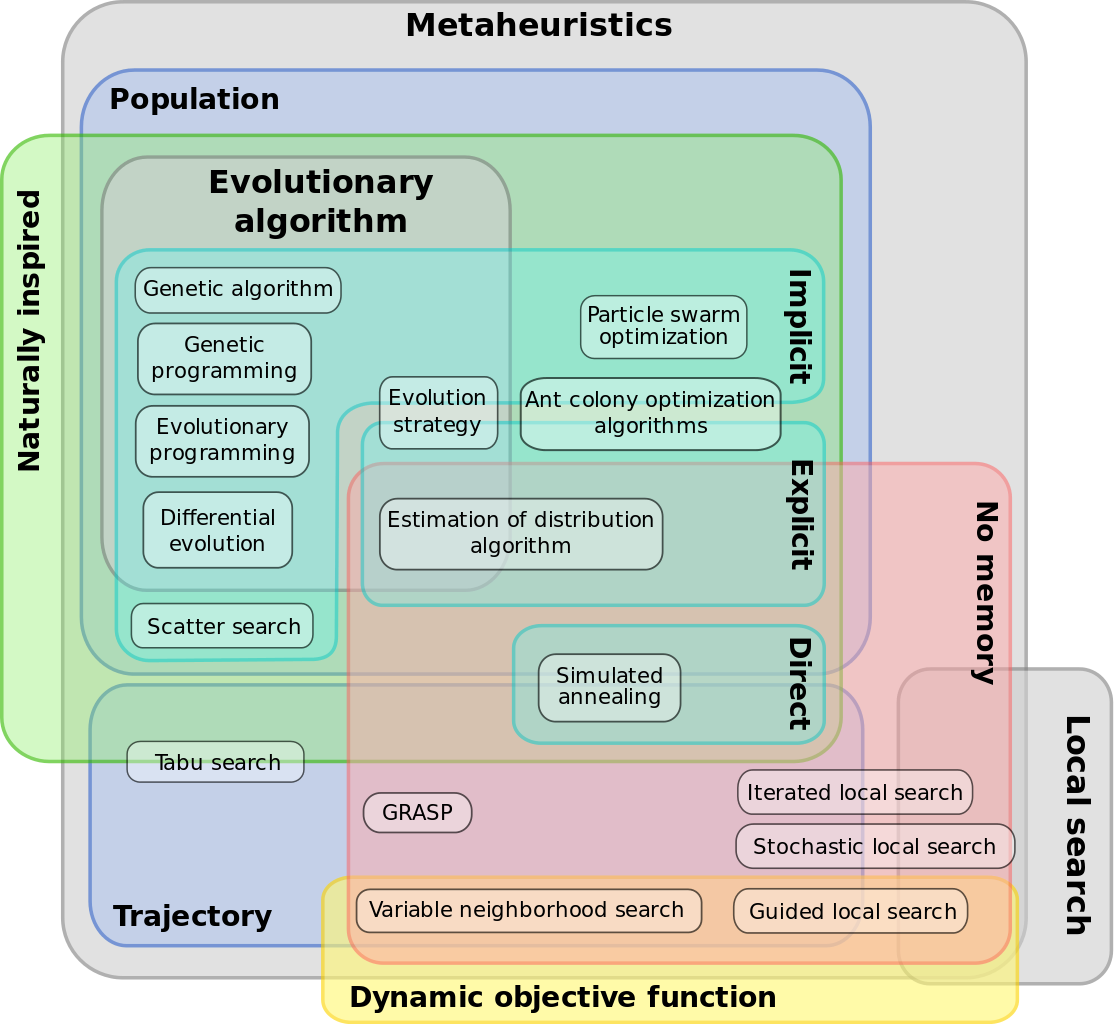
\includegraphics[width=0.7\textwidth]{graphics/Background/Metaheuristics_classification}
	\caption{Meta-heuristics Classification.}
	\label{BG: MH classification}
\end{figure}

As an example, authors in~\cite{birattari2001classification} classification review highlight following characteristics:
\begin{itemize}[itemsep=8pt]
	\item The \textbf{walk-through search space method} could be either trajectory based or discontinuous. The former one corresponds a closed walk on the neighborhood where such prominent examples as \textit{Iterated Local Search}~\cite{lourencco2003iterated} or \textit{Tabu Search}~\cite{glover1989tabu} do exist. The later one allows large jumps in the search space with many MH exemplars, such as \textit{Variable Neighborhood Search}~\cite{hansen2003variable} and \textit{Simulated Annealing}~\cite{kirkpatrick1983optimization}.
	
	\item The \textbf{number of concurrent solutions} could be either single or multiple (population). Such approaches as Tabu Search, Simulated Annealing or Iterated Local Search are examples of former and Evolutionary Algorithms~\cite{eiben2015evolutionary}, Ant Colony Optimization~\cite{dorigo2007ant}, Particle Swarm Optimization~\cite{kennedy1995particle} are instances of later.
	
	\item From the \textbf{memory usage} perspective, we distinguish those approaches which do and don't utilize memory. The Tabu Search explicitly use memory in forms of tabu lists to guide the search, but the Simulated Annealing is memory-less.
	
	\item \textbf{Neighborhood structure} could be either static or dynamic. Most local search algorithms, such as Simulated Annealing and Tabu Search are based on static neighborhood. The Variable Neighborhood Search is an opposite case, where various structures of neighborhood are defined and interchanged while solving an OP. 
\end{itemize}

There are many more classification facets, with are out of this thesis scope. Figure~\ref{BG: MH classification} illustrates the summarized classification including some skipped characteristics and well-known meta-heuristic instances~\cite{wiki_MH_classification}.


\subsubsection{Meta-Heuristics Examples}\label{BG: MH Examples}
Now we shortly describe some prominent and widely used meta-heuristics. The motivation for doing so comes from later usage of them as the LLH in Hyper-Heuristic, described in section~\ref{Impl: LLH}.

\paragraph{Evolutionary Algorithms (EAs).} Evolutionary Algorithms are directly inspired by the processes in nature, described in evolution theory. The common underlying idea in all of these methods is as follows: if we put a population of individuals (Solutions) into an environment with limited resources (population size limit), a competition processes cause natural selection, where only the best individuals survive (compared by the optimization objective)~\cite{eiben2015evolutionary}.

Tree basic actions are defined as operators of EAs: the \textit{recombination} operator that when applied to selected among available in population candidate Solutions (parents) produces new ones (offspring); \textit{mutation} operator applied to Solutions creates a new and very similar one. 
Applying both operators will create a set of new Solutions — the offspring, whose fitness evaluated on TS. After that, the \textit{selection} operator applied to all available Solutions (parents and offspring) for keeping the population size within defined boundaries. This process is repeatedly iterated until some termination criteria fulfilled, for instance maximal iterations counter reached, number of TS evaluations exceed, or Solution with required quality found. The work-flow of EA depicted on Figure~\ref{bg:pic:EAs}.

\begin{figure}
	\centering
	\includesvg{EA}
	\caption{Evolutionary Algorithm Control Flow}
	\label{bg:pic:EAs}
\end{figure}

Well-known examples of EAs include \textit{Genetic Algorithm}~\cite{sastry2005genetic}, \textit{Genetic/Evolutionary Programming}~\cite{koza1992evolution}, \textit{Evolution Strategies}~\cite{beyer2002evolution}, and many other algorithms.

\textbf{Genetic Algorithm} (GA) is the first association coming into mind when you hear words `Evolutionary Algorithms'. GA traditionally has a fixed work-flow: given initial population of \underline{$\mu$} (we underline hyper-parameters here and in other examples of algorithms) usually randomly sampled individuals, the parent selection operator creates pairs of parents where probability of each solution to become a parent depends on its fitness. After that, the crossover operator is applied to each pair with probability \underline{$p_c$} to produce children. Then newly created Solutions undergo mutation operator with independent probability \underline{$p_m$} (hyper-parameter). Resulting offspring perform tournament within selection operator and \underline{$\mu$} survivals replace current population~\cite{eiben2015popular}. Distinguishable characteristics of vanilla GA are usage of following operators: bit-strings Solution representation, one-point crossover recombination, bit-flip mutation and generational (only children survive) selection.

\textbf{Evolution Strategy} (ES) algorithms, in contradiction to GA, are working in a vector space of Solution representation and distinguish \underline{$\mu$} individuals population size and \underline{$\lambda$} offspring generated in one iteration. Often, ES utilizes a very useful feature of \textit{self-adaptation}: changing the mutation step sizes in a runtime. The self-adaptive information is related only to ES, but not to OP under consideration and appended to the individual's chromosome. While the general work-flow for all EAs remains the same, some among underlying operators are changed. Here, parent selection operator take a whole population into consideration, the recombination scheme could involve more than two parents to create one child. To construct a child, \underline{recombination operator} adds alleles from parents in two possible ways: (1) with uniform probability for each parent (discrete recombination), (2) averaging the weights of alleles (intermediate recombination). There are two general \underline{selection schemes}, used in such algorithms: $(\mu,\lambda)$ — discard all parents and selecting only among offspring highly enriching exploration, and $(\mu+\lambda)$ — include predecessor Solutions into selection, a.k.a. \textit{elitist selection}~\cite{eiben2015popular}.

\paragraph{Simulated Annealing (SA).} This is the other type of meta-heuristic, inspired by the technique used in metallurgy to obtain 'well-ordered' solid state of metal. Annealing technique imposes a globally minimal internal energy state and avoids local minimums semi-stable structures. 

The search process in SA treated as the metal with a high temperature at the beginning and lowering it to minimum while approaching the end. %SA algorithm handles the optimization objective as annealing threat the material energy. 
SA starts with initial Solution $S$ creation (randomly or using some heuristic) and temperature parameter \underline{$T$} initialization. At each iteration, new solution candidate $S^*$ sampled within a neighborhood $N(S)$ of current $S$ and the selection criteria evaluated based on $S^*$ quality and $T$ value. $S^*$ replaces $S$ if (1) optimization objective $f(S^*)$ dominates over $f(S)$ or (2) with a probability that depends on quality loose and current $T$ value: $p(T, f(S^*), f(S)) = \exp(-\frac{f(S^*) - f(S)}{T})$. %for minimization OP and $p(T, f(S^*), f(S)) = \exp(-\frac{f(S) - f(S^*)}{T})$. 
At each iteration the temperature parameter $T$ value is decreased following some type of \underline{annealing schedule} also called as \textit{cooling rate}~\cite{boussaid2013survey}. The weak side here is that the quality of each annealing schedule is problem dependent and cannot be determined beforehand, however SA algorithms with parameter control do exist and address this problem by changing the Cooling Rate or temperature parameter $T$ during the search process. Later we shortly review these techniques in section~\ref{bg: parameter control: SA}.


\subsection{Hybrid-Heuristics}
The hybridization of different systems often provides a positive effect — taking the advantages of one system you merge them with odds of other system, thereby getting the best from both of them. The same idea applicable in case of meta-heuristics. Imagine you have two algorithms, biased towards exploration and exploitation respectively. Applying them separately, the expecting results in most cases may be far away from optimal as the outcome of disrupted diversification-intensification balance. But when merging them into, say, repeater stages of hybrid heuristic, one will obtain both advantages of escaping local optima and finding good quality results. 

Most of available hybridization are done exactly with this idea — \textit{staging combination} of two heuristics, one exploration and second exploitation suited for getting outperforming hybrid.

The methods to construct hybrids are mostly defined by the underlying heuristics, thus, to the best of our knowledge, could not be generalized and classified well. One common shared characteristic is usage of \textit{staging approach}, where the output of one algorithm is used as initial state of other. 

As for simple heuristics, we will introduce some examples of performed hybridization in order to give you a better understanding of possible hook parts within algorithms and influence of aforementioned balance onto the search process.

\subsubsection{Hybrid-Heuristics Examples}
\paragraph{Guided Local Search + Fast Local Search~\cite{tsang1997fast}.}
The main focus of \textit{GLS} here is on the Search Space exploration and guidance of process using incubated information. In some sort, \textit{GLS} is closely related to the \textit{Frequency-based memory} used in Tabu Search. During the runtime, \textit{GLS} modifies the cost function of the problem to include penalties and passes this modified cost function to local search procedure. These penalties form memory that characterize a local optimum and guide the process out of it. A local search procedure carried out by the \textit{FLS} algorithm, where the main advantage is quick neighborhood traversal. It is done by braking it up into a number of small sub-neighborhoods, and ignoring those without an improving moves by performing depth first search over these sub-neighborhoods. At some point of time \textit{FLS} reaches the local optimum and passes back the control in \textit{GLS} to repeat the iteration.

\paragraph{Direct Global + Local Search~\cite{syrjakow1999efficient}.}
This hybridization combines mentioned in name optimization strategies into two stages: stochastic global coarse pre-optimization refined by deterministic local fine-optimization. In first stage authors apply one of two described earlier meta-heuristics — Genetic Algorithm, or Simulated Annealing. The transition from Global to Local search happens after reaching the predefined conditions, for instance, when the number of Target System (goal function) evaluations exceeds a boundary, or when no distinguishable improvement was done in the last few iterations. Then, the Pattern Search algorithm~\cite{hooke1961direct} also known as direct/, derivative-free/, or black-box search plays role of Local Search heuristic in this combination. The hybrid-heuristic terminates when Pattern Search converges to local optima.

\paragraph{Simulated Annealing + Local Search~\cite{martin1996combining}.}
After brief explanation of previous two hybrids, an observant reader might make a guess what happens in this particular case, and he will be precisely correct!
Authors named this method `Chained Local Optimization', in other words it is yet another representative of staged hybridization. 
Iteration starts with the current Solution perturbation — 'kick', referring a dramatic change of current position within the search space. After this, some Local Search heuristic applied to intensify obtained Solution. Reaching the local optimum, Local Search pass the control flow back to the Simulated Annealing for acceptance criteria evaluation in order to accept or reject a new Solution, which finishes one iteration.

\paragraph{EMILI~\cite{pagnozzi2019automatic}.}
Easily Modifiable Iterated Local search Implementation (EMILI) is a framework-like system for automatic generation of new hybrid stochastic Local Search algorithms. \textit{EMILI} is a solver for Permutation Flow-Shop Problems (PFSP), also known as Flow Shop Scheduling problems in which performed a search of an optimal sequence of steps to create products within a workshop.
Here authors have implemented both algorithmic- and problem-specific building blocks, defined grammar-based rules for those blocks composition and used an automatic parameter tuning tool \textit{IRACE}~\cite{lopez2016irace} to find a high performing algorithm configurations. The work-flow of \textit{EMILI} could be split onto three steps: (1) adaptation of grammar rules to specific PFSP objective representation type (Make-span, Sum completion times, Total tardiness), (2) generation of all possible hybrid heuristics for each of PFSP type and (3) appliance of iterated racing in \textit{IRACE} to select the best performing hybrid for specific problem type. 

From our perspective, described approach of automatic algorithm generation is direct incumbent of construction Hyper-Heuristics strategies described in upcoming section~\ref{bg: hh}, however we are not authorized to change the system class (from hybrid- to hyper-heuristic) defined by \textit{EMILI} authors.
\todoy{or we can move it into hyper-heuristics?}


\subsection{No Free Lunch Theorem}
A nature question could arise ``If we have all this fancy and well-performing heuristics, why should we put an effort in developing new algorithms, instead of using the existing?'' And the answer to this question is quite simple — the perfect algorithm suited for all OP does not exist and can not exist. 
The empirical research has shown that some meta-heuristics perform better with some types of problems, but poorly with others. In addition to that, for different instances of the same problem type, the same algorithm could result in unexpected performance metrics. Moreover, even in different stages of same problem solving process the dominance of one heuristic over another could change. 

All search algorithms perform exactly the same, when the results are averaged over all possible Optimization Problems. If an algorithm is gaining the performance in one problems class, it loses in another class. This is a consequence of so-called \textbf{No Free Lunch Theorem for Optimization} (NFLT)~\cite{wolpert1997no}.

In fact, one could not predict, how exactly will behave one or another algorithm with problem in hand. A possible and the most obvious way is to probe one algorithm and compare its performance to another one during problem solving process. In this case simple heuristics and meta-heuristics are out of competition, since once you solved the Optimization Problem you probably wouldn't optimize a second time.
Here come \textbf{Hyper-Heuristics} to intelligently pick heuristics that is suitable to problem in hand. We will proceed with their description and how they deal with the NFLT consequences in following section.


\subsection{Hyper-Heuristics}\label{bg: hh}
A lot of state-of-the-art heuristics and meta-heuristics are developed in a complex and very domain-dependent way, which causes problems in an algorithm implementation reuse. It motivated research community to raise the level of generality at which the optimization systems can operate and still provide good quality Solutions for various Optimization Problems. 

The term \textbf{Hyper-Heuristic} (HH) was defined to describe an approach of using some \textit{High-Level-Heuristics} (HLH) to select over other \textit{Low-Level-Heuristics} (LLH) and apply them to solve the \textit{class of Optimization Problems} rather than particular instance. Indeed, scientists report that the combination of different HLH produces better results than if hey were applied separately~\cite{drake2019recent} — note previously discussed hybrid-heuristics.
This behavior can be explained by the nature of search process and how it evolves in time. When you apply a heuristic, it sooner or later converge to some extreme point, hopefully global optimum. But it is `blind' to other, not visited regions in the Search Space. Changing the trajectory of investigation by (1) drastically varying the Neighborhood, (2) changing the strategy of Neighborhood exploration and exploitation could (1) bring you to those previously unreachable zones (2) in more rapid ways. However, usually it is hard to predict how one LLH will behave in every stage of the search process in comparison to another. In Hyper-Heuristics, this job was encapsulated into the HLH and performed automatically. 

In~\cite{moriarty1999evolutionary} authors made infer that Hyper-Heuristics can be viewed as a form of Reinforcement Learning, which is a logical conclusion especially if we rephrase it to \textit{Hyper-Heuristics utilize Reinforcement Learning methodologies}.

\begin{figure}
	\centering
	\includesvg{HH}
	\caption[Hyper-Heuristics]{Hyper-Heuristics.}
	\label{bg:pic:HH}
\end{figure}

The new concept which implicitly was used in Meta-Heuristics, but explicitly pointed out in Hyper-Heuristics is the \textbf{Domain Barrier} (Figure~\ref{bg:pic:HH}\footnote{Icons from \href{https://thenounproject.com/}{thenounproject.com}}).
As we told previously, HH do not tackle an OP directly, but use LLH instead. This means, that usually HH are minimally aware of the domain details, such as what are data types, relationships, etc. within a domain. This information rather encapsulated in LLHs, thus HHs could be used to broader range of Optimization Problems.

With this idea, many researchers started to create not only Hyper-Heuristics to tackle a concrete optimization problem class, but also frameworks with building blocks for their creation.


\subsubsection{Classification}
Although, the research in Hyper-Heuristics field is actively ongoing, many algorithm instances were already created and some trials to organize approaches were conducted in~\cite{ryser2014review,drake2019recent,burke2019classification}.

Researchers in their surveys classify HHs by different characteristics, some of which overlap, but it also happens that important (from our perspective) features were not highlighted in all works. 

In this section we present the union of those important Hyper-Heuristics classification facets to better justify the goal of this thesis.

We begin with the two broadest classes, which differentiate HH \textbf{routine}, also called as \textbf{nature of High-Level-Heuristic Search Space}~\cite{burke2013hyper,burke2019classification,drake2019recent}.
The first class are Hyper-Heuristics to \textit{select} Low-Level-Heuristic, in other words \textit{Selection Hyper-Heuristic}. All our previous references to Hyper-Heuristics were made this concrete type. These algorithms operate in the Search Space, defined by complete and rather simple Low-Level-Heuristics that solve Optimization Problem. The task of HLH here is to pick the best suited LLH (or sequence of LLHs) based on available prior knowledge and apply it to OP underway. Note, that staging Hybrid-Heuristics could be viewed as Solutions of Selection HHs.
Hyper-Heuristics of the second class seek to \textit{construct} LLH following some predefined receipt and using the atomic components of other heuristics as Lego bricks. The other commonly used name here is \textit{Construction Hyper-Heuristics}. These approaches often lead to creation of new and unforeseen heuristics that are expected to reveal good performance while solving the problem in hand.

Next, the distinction in \textbf{nature of Low-Level-Heuristics Search Space} arises. 
In other words: ``How does the LLH derive Solutions for the OP?'' Authors in~\cite{burke2013hyper,burke2019classification,drake2019recent} distinguished \textit{construction} LLHs where Solution creation happens each time from scratch and \textit{perturbation} LLHs where new Solutions created from parts of already existing ones.

The other broadly used characteristic is the \textbf{memory usage method}. 
From this perspective we distinguish Hyper-Heuristics in which the learning happens \textit{on-line}, \textit{off-line} or learning mechanisms are \textit{not present} at all~\cite{ryser2014review,burke2019classification}.
\begin{itemize}[itemsep=8pt]
	\item In \textbf{on-line} case, the HH derives an information, used to select among LLH, while those LLH are solving the problem.

	\item In \textbf{off-line} case, the learning happens before solving concrete Optimization Problem. Here one should first train an HH solving other homogeneous problem instances by underlying LLHs (off-line learning phase). After that, the HLH will be able to choose among LLHs, thus be applicable to problem in hand (on-line use phase). Note, that this approach also requires creation of meta-features extraction mechanism and its application to every Optimization Problem.

	\item There exist also \textbf{mixed} cases, where learning happens first in off-line and later also in on-line phase. Definitely it is a promising (in terms of results quality) research direction, despite it high complexity.
	
	\item In the last case \textbf{no learning} mechanisms present, therefore HLH here performs some sort of Random Search over LLH Search Space. At first sight, it may look like weak approach, but looking onto Variable Neighborhood Search Meta-Heuristic we would doubt it.
\end{itemize}


%Yet another faced of Hyper-Heuristics classification is the way of assigning \textit{hyper-parameters} (here we use parameters and hyper-parameter concepts interchangeably) for LLHs, or their components~\cite{drake2019recent}. We analyzed surveys and find out that some researchers do not explicitly differentiate approches with respect to nature of parameter settings~\cite{ryser2014review,burke2013hyper,burke2019classification}, while other do~\cite{drake2019recent}:
%\begin{itemize}
%	\item In \textbf{static} assignment, the underlying heuristics use provided beforehand (usually default) hyper-parameters and do not change them while solving the problem in hand.

%	\item The \textbf{dynamic} case uses some kind of rule for parameters changing, specified in advance.

%	\item There exist also an \textbf{adaptive} approach, in which HH assigns the parameters for LLH as the response to the learning process. In some sort, it is similar to the parameter control techniques used in Meta-heuristics.
	
%	\item And finally, a \textbf{self-adaptive} approach where underlying LLHs comprise \textit{parameter control} techniques, thus search for the best solution for OP and own parameter settings simultaneously.
%\end{itemize}


For more detailed analysis, description, other classification facets and respective Hyper-Heuristic examples we encourage reader to look into resent classification and surveying researches~\cite{burke2003hyper,ryser2014review,drake2019recent,burke2019classification}.

\subsubsection{Hyper-Heuristics Instance Examples}\label{bg: hh examples}
\paragraph{Hyper-Heuristic for Integration and Test Order Problem~\cite{guizzo2015hyper}.} \textit{HITO} is an example of generational HH. LLHs in this case are presented as a composition of basic EAs operators — crossover and mutation forming multi objective evolutionary algorithms (MOEA). HH selects those components from $jMetal$ framework~\cite{durillo2011jmetal} using interchangeably Choice Function (in form of weighted linear equation) and Multi Armed Bandit based Heuristic to balance exploitation of good components and exploration of new promising ones.


\paragraph{Markov Chain Hyper-Heuristic~\cite{mcclymont2011markov}.} \textit{MCHH} is an on-line selective Hyper-Heuristic for multi-objective continuous problems. It utilizes reinforcement learning techniques and Markov Chain approximations to provide adaptive heuristic selection method. While solving an OP, \textit{MCHH} updates prior knowledge about the probability of producing Pareto dominating Solutions by each underlying LLH using Markov Chains, thus guiding an LLH selection process. Applying on-line reinforcement learning techniques, this HH adapts transition of weights in the Markov Chains constructed from all available LLHs, thus updating prior knowledge for LLH selection.


\subsubsection{Hyper-Heuristics Frameworks Examples}\label{bg: hh fw examples}
\paragraph{Hyper-Heuristics Flexible Framework~\cite{ochoa2012hyflex}.} \textit{HyFlex} is a software skeleton, built specifically to help other researchers creating Hyper-Heuristics. It provides the implementation of components for 6 problem domains (Boolean Satisfiability, Bin Packing, Personnel Scheduling, Permutation Flow Shop, Traveling Salesman and Vehicle Routing problems), such as problem and solution descriptions, evaluation functions and adaptations for set of Low-Level-Heuristics. The set benchmarks and comparison techniques to other built HHs on top of \textit{HyFlex} are included to framework as well. 

The intent of \textit{HyFlex} creators was to provide Low-Level features that enable others to focus directly on High-Level-Heuristics implementation without need to challenge other minor needs. It also brings a clear comparison among created HLH performance, since the other parts are mostly common. From the classification perspective, all derivatives from the \textit{HyFlex} framework are Selection Hyper-Heuristics, however they utilize different learning approaches. Algorithms, built on top of \textit{HyFlex} framework could be found in many reviews~\cite{misir2012intelligent,ryser2014review,drake2019recent} or on the CHeSC 2011 challenge website\footnote{\href{http://www.asap.cs.nott.ac.uk/external/chesc2011/}{Cross Domain Heuristic Search Challenge website: asap.cs.nott.ac.uk/external/chesc2011/}} (dedicated to choosing the best HH built on top of \textit{HyFlex}).

Along with \textit{HyFlex}, a number of hyper-heuristic-dedicated frameworks is growing, some of them are under active development while others are abandoned:
\begin{itemize}[itemsep=8pt]
	\item \textbf{Hyperion}~\cite{swan2011hyperion} is a construction hyper-heuristic framework aiming to extract information from OP search domain for identification of promising components in form of object-oriented analysis.
	
	\item \textbf{hMod}~\cite{urra2013hMod} framework allows not only to rapidly prototype an algorithm using provided components, but also to construct those components using predefined abstractions (such as $IterativeHeuristic$). In current development stage, developers of \textit{hMod} are focusing on creation of development mechanisms rather than providing a set pre-built heuristics. 
	
	\item \textbf{EvoHyp}~\cite{pillay2017evohyp} framework focuses on hyper-heuristics created from evolutionary algorithms and their components. Here authors enable framework users to construct both selection and generation HHs for both construction and perturbation LLHs types.
\end{itemize}


\subsection{Conclusion on Heuristic Solvers}
To conclude our review on Heuristic approaches for solving Optimization Problems, we shortly remind you pros and cons of each heuristic level.

On the basis remain Simple Heuristics with all their domain-specific knowledge usage and particular tricks for solving problems. Usually, they are created to tackle a concrete problem instance in hand applying simple algorithmic approach. The simplicity of application and usually fast runtime paid back by medium results quality.

On the next level inhabit Meta-Heuristics. They could be compared with more sophisticated Solutions hunters which could not only charge directly, but also take a step back when stuck in a dead end. This additional skill enables them to survive in new and complex environments (Optimization Problems), however some adaptations to understand a concrete problem and parameter tuning for better performance still should be performed.

Among with MHs exit Hybrid-Heuristics. There is nothing special here, they just took some survival abilities from several Meta-Heuristics hoping to outperform and still requiring adaptation and tuning. In some cases this hybridization provides it advantage, but as the time shows, they did not force out MHs. Those we can conclude that the provided balance between development effort and exposed results quality not always assure users to use them.

Finally, the chosen ones that lead the others, Hyper-Heuristics are on the upper generality level. 
Operating by the other Heuristics, HHs analyze how good former are and make use of this knowledge by solving the concrete problem using those best suited Heuristics. Imposing such great abilities, Hyper-Heuristics tackle not only the concrete optimization problem, but entire class of problems.


\section{Setting Algorithm Parameters}\label{bg: section Parameters Setting}
The most of existing learning algorithms expose some parameter set, needed to be assigned before using this algorithm. Modifying these parameters, one could change the system behavior and possible result quality.

When we are talking about the problem of settings the best parameters, following terms should be refined explicitly:
\begin{enumerate}
	\item \textbf{Target System (TS)} is the subject which parameters are undergoing changes. Simply, it could be a heuristic, machine learning algorithm or other system.
	\item \textbf{Parameter} is one of exposed by TS setting hooks. It should be described in terms of its type and possible values.
	\item \textbf{Configuration} is the unique combination of parameter values, sufficient to run TS.
	\item \textbf{Search Space} is the set of all possible Configurations for defined Parameters.
\end{enumerate}

In this thesis we use notions of \textit{Parameter} and \textit{Hyper-Parameter} (HP) interchangeably, since the approaches discussed in this section are generally applicable also in Machine Learning cases. For instance, consider Neuron Network (NN). Hyper-parameters in this case will specify the structure (number of hidden layers, units, etc.) and learning process (learning rate, regularization parameters values, etc.) of network and changing them dramatically affect performance and results.

One frequent incumbent of Optimization Problems is \textbf{Parameter Settings Problem} (PSP) — searching of hyper-parameter values that optimize some characteristic of TS. When talking about NN example, PSP could be defined as task of maximization network accuracy in given dataset (Single Objective PSP). Taking into account a number of TS characteristics simultaneously, such as training time and prediction accuracy PSP transforms into Multi-Objective PSP.

The same applies to heuristics: proper assignment of hyper-parameters has a great impact on exploration-exploitation balance and thus on overall algorithm performance.

Up until now there were formalized many approaches for solving task of settings hyper-parameters. 
One of the simplest and error-prone ways is just trusting your (or someones else) intuition and using those parameters that seems more or less logical for particular system under the problem instance. People quickly abandoned it in favor of automatic approaches, fortunately novel computational capacities easily provide a possibility for it. These automatic methods later could be split onto \textit{off-line or parameter tuning} and \textit{on-line or parameter control} techniques.


\subsection{Parameter Tuning}
Roughly speaking, the off-line approach is a process of traversing the search space of hyper-parameters and evaluating TS with these parameters on some set of toy problems. After finishing this process, the best found HPs are later used to solve new, unforeseen problem instance.

In this part of thesis we briefly outline existing automated approaches for parameter tuning illustrating them on a figure~\ref{bg: fig:automated parameter tuning approaches}\footnote{Original graphics are taken from~\cite{koch2017automated}}. In this example, the TS exposes two parameters: $X_1$ and $X_2$. Each graphic shows dependencies between $X_1$ (horizontal axis) and $X_2$ (vertical axis) values and the subject of optimization along those axes (here depicted the maximization case). The best found configuration by each approach is highlighted in pink.

\begin{figure}
	\centering
	\begin{subfigure}[b]{0.25\linewidth}
		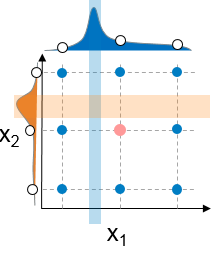
\includegraphics[width=\linewidth]{graphics/Background/hyperparameter-grid-search.png}
		\caption{Grid.}
		\label{bg: fig:automated parameter tuning approaches: grid}
	\end{subfigure}
	\begin{subfigure}[b]{0.25\linewidth}
		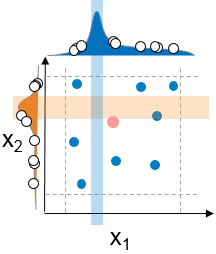
\includegraphics[width=\linewidth]{graphics/Background/hyperparameter-random-search.png}
		\caption{Random.}
		\label{bg: fig:automated parameter tuning approaches: random}
	\end{subfigure}
	\begin{subfigure}[b]{0.25\linewidth}
		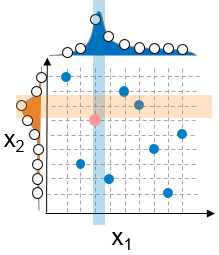
\includegraphics[width=\linewidth]{graphics/Background/hyperparameter-learning-search.png}
		\caption{Learning.}
		\label{bg: fig:automated parameter tuning approaches: learning}
	\end{subfigure}
	\caption{Automated Parameter Tuning Approaches.}
	\label{bg: fig:automated parameter tuning approaches}
\end{figure}

\paragraph{Grid Search Parameter Tuning.} It is a rather simple approach for searching parameters. Here the original search problem is relaxed and later solved by brute-force algorithm. The set of all possible configurations (parameter sets) for relaxed problem is derived by specifying a finite number of possible values for each hyper-parameter under consideration. After evaluating all configurations on TS, the best found solution is reported. As you can see, this approach could skip promising parts of search space (Figure~\ref{bg: fig:automated parameter tuning approaches: grid}).

\paragraph{Random Search Parameter Tuning.} This methodology relies on random (often uniform) sampling of hyper-parameters and their evaluation on each iteration. At first sight, it might look unreliable to chaotically traverse the search space. But empirical studies show that with growing number of evaluations this technique starts to outperform grid search~\cite{bergstra2012random}: compare the best configurations (highlighted in pink) found by grid (Figure~\ref{bg: fig:automated parameter tuning approaches: grid}) and random search (Figure~\ref{bg: fig:automated parameter tuning approaches: random}) techniques.

\paragraph{Model Based Search Parameter Tuning.} In the most cases, the dependencies between tuned parameter values and optimization objective do exist and can be utilized for hyper-parameter tuning. By predicting which parameter combinations lead to better results, model-based tuning could make precise guesses. As it showed on Figure~\ref{bg: fig:automated parameter tuning approaches: learning}, at the beginning, this approach behaves as random search, but after accumulating enough information, learning algorithm starts making more precise guesses, which in contrast to previously described model-free approaches is desirable and more robust.

Naturally, this optimization problem could be tackled by almost every discussed here approach, however taking into account the facts that (1) TS here in most cases is a \textit{black-box} we eliminate exact and approximate solvers, (2) the evaluation cost is huge, thus it is not desirable to apply any of described above heuristics directly.

With this idea in mind, researchers started to (1) create  Bayesian optimization algorithms that traverse the search space more efficiently and (2) build models that could recreate the dependencies between parameters and objective values, a so-called \textit{surrogate models}. While the former direction is nothing else but an enhancement to already existing optimization techniques, the later one is crucial for problems where objective is expensive to evaluate.
The later is some sort of enhancement used in combination with former enabling you to simulate evaluation of real system instead of expensive direct evaluations. Still, it is a common approach to combine previously reviewed search space traversal techniques, such as Evolutionary Algorithms, Simulated Annealing, Tabu Search with surrogate models for optimization.


\subsection{Systems for Model-Based Parameter Tuning}\label{bg: parameter tuning expamples}
The parameter tuning is an obligatory task when the maximum system performance is a mast-have requirement and should be performed at the design time.
Novel tuning approaches are usually built in form of frameworks with exposed hooks for attaching the system under estimation.

Since, the Target System evaluations here supposed to be extremely costly, thus parameter tuning frameworks are trying to utilize every single bit of information from evaluations by building surrogate models and using Bayesian optimization approaches is obligatory.

In this section we review some among existing open-source parameter tuning systems from following perspectives:
\begin{itemize}[itemsep=8pt]
	\item \textbf{Conditional parameters support} is (1) a provided for user and (2) handled by tuning system ability to describe conditional dependencies between hyper-parameters. As an example, imagine \textit{crossover type} parameter of Genetic Algorithm that can take only some specific values: \textit{Partially Mapped Crossover ($PMX$)}, \textit{Cycle Crossover ($CX$)}, etc. Binding concrete crossover type, one will be required provide parameters for this crossover type, but eliminate respective parameters for other crossover types. This type of dependency could be described in form of parent-child relationship, however other types of dependencies also exists.
	
	\item \textbf{Parameter types support} is one of the basic usable tuning systems requirements. More concretely, Target System parameters could be not only numerical (integer or fractional), but also categorical in form of strings, boolean values, etc. Considering categorical data types, they could be either \textit{nominal} (depict only possible atomic values) or \textit{ordinal} (implies also value comparison, but no distance notion). For instance lets again analyze parameters of Genetic Algorithm: population size — numerical integer in range $[1...\inf)$, mutation probability — numerical fractional $[0...1]$, crossover type — categorical nominal ${PMX, CX}$. Indeed, we could treat population size as a set of finite values ${10, 100, 1000}$ — categorical ordinal parameter type.
	
	\item \textbf{Extensibility} is crucial when someone would like to try a new promising and intriguing learning algorithm for guiding a search, that was not available in parameter tuning system yet. Practically, one may need not only new learning algorithm, but some other features like non-trivial stopping criterion, tools for handling stochastic behaviors, or different strategies for random sampling (which are utilized while tuning system is learning before making a prediction).
	
	\item \textbf{Parallel Evaluations} required for utilizing available computing resources that could scale horizontally, thus providing simultaneous evaluation of multiple Configurations which speeds-up the learning process.
\end{itemize}

Among reviewed systems we could distinguish ones that were created directly to face the parameter tuning problem and the others that are more generic optimizers but still applicable in parameter tuning cases.
A concrete optimizer will be usable for searching the parameters, if it exposes several features. First, it must consider optimization function evaluation to be expensive and tackle this problem explicitly. For instance, using surrogate models or other Target System (TS) approximations. Next, potential tuner should be able to tackle dependencies and conditions among parameters.

\subsubsection{SMACv3~\cite{hutter2011sequential}}\label{bg: smac}
Sequential Model-based Algorithm Configuration is a system for parameters tuning, developed by the AutoML research group (here we review \textit{SMACv3}). 

In their researches, scientists generalized the process of parameter tuning under the term \textit{Sequential Model-Based Optimization} as iterations between steps of (1) fitting models and (2) using them to choice next Configurations for evaluation. 
We found that this term greatly formalizes all existing (to the best of our knowledge) parameter tuning approaches and should be used as a distinguishing characteristic of tuning algorithms (since they naturally could be applied not only to parameter tuning problems).

\textit{SMAC} is an extension introducing learning models and sampling mechanisms based on them to previously existing Random Online Aggressive Racing (\textit{ROAR}) mechanism. Authors showed that the machine learning mechanisms and regression models in particular are applicable not only for tuning parameters, but also for optimizing any expensive black-box functions in general (playing the role of surrogate model). 

The development of this system was motivated to tackle existing limitations of all published SMBO approaches, namely expanding an applicability not only to numerical, but also to categorical parameters and optimizing target algorithm not only on single, but on number of problem instances (benchmark set of problem instances) to reduce the influence of the variance.

A routine in \textit{SMAC} could be imagined as iterated application two tree steps: (1) building learning model, (2) using it for making choices which Configurations to investigate next and (3) actual evaluation of sampled Configurations.

The evaluation (3) here carried out by original ROAR mechanism in which evaluation of each new candidate Solution continues until enough data (from benchmark set of problem instances) obtained to either replace current Solution or reject candidate. In contrary to original, model-less ROAR, \textit{SMAC} at step (1) builds regression random forest — an instance of machine learning algorithm~\cite{breiman2001random}. The usage of regression decision trees (which form the forest) motivated by known fact that they fit well to categorical data and complex dependencies in general. Later, at step (2) the Iterative Local Search (ILS) heuristic applies in combination with \textit{Expected Improvement} (EI) evaluation (form of Bayesian optimization)~\cite{shahriari2015taking}. ILS starts on the best previously found Configuration and traverses its Neighborhood distinguishing between neighboring Configurations using EI and regression model built at step (1). EI is large for those Configurations, which has low predicted cost and for those, with high uncertainty in results, thus naturally providing exploration-exploitation balance~\cite{jones1998efficient}.

Exposing such a great learning capabilities and using Expected Improvement technique that guarantees converging to global optimum given enough time, the major drawback in this system is lack of flexibility to include conditional dependencies between parameters into sampling process. 

In fact, used here search space representation framework \textit{ConfigSpace}\cite{configspace} is able to specify dependencies among hyper-parameters. However, to the best of our knowledge, during the Configuration sampling those conditions are not taken into account and could be broken thus resulting in illegal parameter combination. Those cases are handled and broken Configurations are rejected by \textit{ConfigSpace}, but we believe that in case of `sparse' search spaces (where significant amount of parameter combinations are restricted by conditions) this approach could lead to ineffective sampling and great struggling in system predictive abilities. Unfortunately, we did not find any officially published empirical studies of such cases and can only make guesses based on own intuition. However, the \textit{SMACv3} developers advises for operation in such cases~\footnote{Visit GitHub repository of \textit{SMACv3} for more info~\url{https://github.com/automl/SMAC3/issues/403}} could serve as an evidence to correctness of our assumptions. One of possible solutions here could be the use of conditional-aware neighborhood definition in ILS (currently sampling is performed in regular Gaussian distribution). 

\textit{ROAR} mechanism is the derivative from \textit{FocusedILS} algorithm (solver in \textit{ParamILS} parameter tuning framework~\cite{hutter2009paramils}) where each evaluation of new candidate Solution on problem instance performed sequentially. Since the \textit{ROAR} evaluation strategy is applied at step (3), we conclude that the utilization of available computation capabilities is, possibly, another drawback of \textit{SMACv3} framework.


\subsubsection{IRACE~\cite{lopez2016irace}}\label{bg: irace}
The first system under analysis is an implementation if Iterated Racing Algorithm~\cite{birattari2010f} in \textit{IRACE} hyper-parameter tuning package.

The underlying methodology is somehow similar to one implemented in \textit{SMACv3} and consists of three main steps: (1) sampling new Configurations using prior knowledge, (2) finding the best ones among sampled using racing algorithm and (3) updating the prior knowledge to bias future samples in (1) towards better Configurations. 
Prior knowledge here represented as probability distributions for each parameter independently (truncated normal and discrete distributions for numeric and categorical hyper-parameters respectively).% During update step (3), the probability distributions are increased for those values, where the best Configurations were found.

Iterated racing step (2) here is a process of running Target System using sampled Configuration on a set of problem instances. After solving each instance, the statistically worse-performing Configurations are rejected and racing proceeds with remaining ones. This process continues until reaching the required number of survivals or after solving a requiring amount of problem instances (in this case all remaining Configurations are considered to be good). 

\textit{IRACE} supports various data types, such as numerical or categorical and the possibility of conditions description as well. While the problem of data types solved by different underlying distributions, the conditional relationships are handled by the dependency graphs. During sampling (1), first are sampled non-conditional and only afterwards, if respective conditions are satisfied, sampled dependent parameters. 

% TODO: probably, move to implementation part.
The framework highly relies on racing algorithm for parallel evaluations and on \textit{Friedman test}~\cite{conover1980practical} or alternatively \textit{paired t-test} for statistical analysis of Configurations, thus it is static in terms of variability and extensibility of learning mechanisms. 
In terms of parallel evaluations, the algorithm utilizes all available resources at the beginning of each racing step, however as the process continues, fewer evaluations are executed in parallel those available resources are idling and not utilized optimally at all steps of algorithm.


\subsubsection{BOHB~\cite{falkner2018bohb}}\label{bg: bohb}
While \textit{SMAC} outperforms and partially reuses decisions done in \textit{ParamILS}, \textit{BOHB} (Bayesian Optimization combined with HyperBand) is the parameter tuning tool that outperforms \textit{SMAC} and was suggested by the same AutoML research group.

As it stated in name, the \textit{SMBO} routines in this framework are carried out with mainly two algorithms: learning (1) and Configurations sampling (2) done by Tree Parzen Estimator (TPE) — Bayesian Optimization technique, while evaluation of sampled Configurations and their comparison are carried out by HyperBand (HB) algorithm.

The TPE instead of na\"ive Gaussian Processes-based (GP BO) Bayesian Optimization and Expected Improvement evaluation, was motivated by better dimensional scaling abilities and internal support of both numerical and categorical data types (however, some minor transformations are still required). 
Unlike vanilla BO, where the optimization done by modeling results distributions given Configuration parameters, TPE builds two distributions of parameters splitting Configurations into two sets according to their `goodness' and later proposing those parameters with high probability to be in `good' distribution and simultaneously low probability to be in `bad' distribution. For more detailed explanation we refer to TPE description, given in~\cite{bergstra2011algorithms}.

The central part of \textit{BOHB}, namely HyperBand is a promising multi-armed bandit strategy for hyper-parameter optimization~\cite{li2017hyperband} in which the \textit{budget} for Configurations evaluation is defined beforehand and divided into iterations. The role of budget could play any control parameter that denotes the accuracy of Configuration evaluation by TS, where estimation with the maximum budget gives you the most precise Configuration evaluation while minimum amount of budget results in the least accurate approximation of Configuration evaluation result.
Running examples of budget could be the number of iterations in iterative algorithm, epochs to train the neuron network or number of problem instances from benchmarking set.

As the result, requirements arise for TS to expose and support budget usage as expected in \textit{BOHB}.

At each iteration, HB randomly samples a number of Configurations which, in fact, decreases for later iterations while the amount of budget remains the same. As the outcome, first iterations of HB are full of coarse-grain evaluated Configurations, while later iterations produce higher number of more accurate measurements. Each iteration of HB is split to number of Successful Halving (SH) procedure executions which drop (usually $\frac{2}{3}$) badly performing Configurations. As one could expect, since the number of measured Configurations in each iteration decreases, the amount of SHs execution drops too, thus the remaining Configurations are evaluated more precisely.

The binding of HyperBand and Bayesian Tree Parzen Estimator made is several places. Firstly, the learning models are updated each time when new results are available for every budget value. Next, at each iteration of HB, TPE model is used for sampling new Configurations. Note that \textit{BOHB} uses models, built on results obtained with the largest budget only. This decision leads in more precise predictions in the later stages of parameter tuning process.

The drawback of this system lays in the way of handling conditions between hyper-parameters. Distributed HyperBand implementation on Steroids (HpBandSter)~\footnote{GitHub repository: \url{https://github.com/automl/HpBandSter}} is a \textit{BOHB} particular implementation uses \textit{ConfigSpace} framework (as \textit{SMACv3}) for Configuration Space definition. As we discussed in \textit{SMACv3} description (section~\ref{bg: smac}), \textit{ConfigSpace} naturally allows to encode the dependencies and conditions among parameters. As authors stated, the TPE learning models are also able to learn these dependencies implicitly by shrinking the densities for forbidden parameters (actually those parameter values are still added to models by \textit{imputation} mechanism where default values are used for forbidden parameters). However, consider a case of two Configurations $C_1$, $C_2$ appearance such that some parameter $P_i$ is forbidden in $C_1$, but not in $C_2$, which will break the densities and as a consequence, the prediction performed using such distributions will often result in Configurations with violated parameter dependencies within `sparse' search spaces, hurting the performance and accuracy of sampling. The actual number of such cases could vary dramatically in `sparse' Search Spaces, thus probability distributions estimated by KDEs will not reflect the reality.


\subsubsection{BRISEv2~\cite{brise2spl}}
The great part of software potential lays not only in its ability to tackle a problem in hand, but also on the general usability and adaptivity to unforeseen tasks.
Here we review BRISE of version 2\footnote{GitHub repository: \url{https://github.com/dpukhkaiev/BRISE2/releases/tag/v2.3.0}}, since the very early BRISE versions (major 1~\cite{brise1monolite}) were more monolithic and hard to apply for parameter tuning problem in hand.

While designing this system, authors were focused on learning mechanisms for parameter prediction and overall system modularity as well.
Being a Software Product Line, BRISE was designed as a set of interacting components (nodes) each acting according to its own specific role. 
The system could be viewed from two perspectives. One is general outline of all available nodes and the other is analysis of~\textit{main-node} concretely.

Before reviewing each part, it is worth to justify formalized in system terms. Note, that they are pretty the same as we defined above, but here most of them also have been implemented in form of classes.
\begin{enumerate}
	\item \emph{Experiment} denotes a complete run of BRISE, for instance parameter tuning session. Handles such information as BRISE Experiment Description (JSON-like specification of parameter tuning procedure), all evaluated during session configurations and derived from description search space.

	\item \emph{Configuration} is a combination of input Parameter values for target system (or algorithm) under evaluation. It could be evaluated several times (to obtain statistical data), thus contain number of \emph{Tasks} and compared against other Configurations.

	\item \emph{Parameter} is a meta-description of concrete Configuration part and a building block for Search Space, defines a set or range of possible values. 

	\item \emph{Search Space} comprises all Parameters and their dependencies, could verify the validity of Configuration.

	\item \emph{Task} is an evaluation of TS under provided Configuration for statically specified in Description scenario.
\end{enumerate}

From a birds eye view perspective, BRISE consists of \textit{main-node} as the system backbone, several \textit{worker-nodes} as target algorithm runners under provided Configurations, \textit{worker-service} to distribute tasks load between set of worker-nodes, \textit{front-end-node} to control and report optimization process on a web-page, and non-obligatory \textit{benchmark-node} that could be handy for executing and analyzing number of Experiments.

To use BRISE for parameter tuning, one should (1) construct an Experiment and Search Space json-like descriptions and (2) add the respective function for target system evaluation in \textit{workers} with provided Task. All the rest will be carried out by system.
% TODO: we deffinitely should formalize Tasks, since this entry is exposed to user (it should parse it to retrieve prameters as well as add results).

From our perspective, the advantage of BRISE over other systems comes from the design of \textit{main-node}. It is a set of operating core entities (Experiment, Search Space and Configuration) with other non-core entities exposed to user for variability, such as surrogate models, termination criteria, outliers detectors, repetition strategies, etc. Naturally, a number of implementations are provided out-of-box for all variable entities. For instance, two prediction models: ridge regression with polynomial features and TPE BO; several termination criteria: wall-clock timeout, exceeding number of evaluated Configurations, absence of improvement and others. Using different combinations entities, one could obtain the system with desired behavior or even further, supply own learning models, sampling plans, enhance termination logic, etc.

As every other system, BRISE also has flaws. Talking about the search space representation, BRISE relies on ConfigSpace module~\cite{configspace} which is also used SMACv3 and BOHB frameworks. The predictive models are acting pretty the same, so all previous claims are also valid here — it is hard to apply BRISE in cases of sparse Configurations spaces.


Generally, the biggest disadvantage of Parameter Tuning defined by the fact, that it usually requires large number of target algorithm runs to evaluate its performance with different settings.
On opposite site, the parameter control approaches are solving this issue but the drawback lays in their universality.


\subsection{Parameter Control}\label{bg: parameter control}
One advantageous characteristic of the system is its ability to adapt in runtime.
It could happen, that tuned algorithm performs well in early beginning of new problem solving, but later could struggle hard while the other configuration may result in opposite behavior. It could be caused by various reasons, and it is usually hard to tell, which of them you are facing at concrete moment. 

In contrast to parameter tuning, where optimal parameters first were searched and only later applied to problem in hand, the parameter control is an approach of searching the best system configuration, while solving the problem in hand. It also could be expressed as the ability of system to react on changes in the solving process, in other words it is known as \textit{on-line} version of parameter tuning. The drawback of this approach lays in lack of generality, since  often the parameter control technique is algorithm dependent.

Searching the examples of parameter control for heuristics, one definitely will find himself exhausted to enumerate all proposed methodologies for evolutionary algorithms, since the origins of this idea lay in EAs~\cite{karafotias2014parameter}. However, techniques for other meta-heuristics do exist too.
As far as we know, the approach to adapt parameters mostly depends on concrete algorithm instance, thus it is hard to present a general classification of approaches for all algorithms, but it could be done for each particular family.

The only one brute classification facet we able to distinguish is the type of control mechanism, where \textit{deterministic} (following a predefined schedule) and \textit{adaptive} (assign parameter values upon received feedback) types are distinguishable.

We provide an insight of parameter control by reviewing some examples among existing adaptation strategies in meta-heuristics.
Generally speaking, authors reported significant improvements in optimization performance for all mentioned control mechanisms in every heuristic. For more comprehensive review of recently published parameter control strategies in meta-heuristics we encourage reader to examine~\cite{huang2019survey}.

\subsubsection{Parameter Control in Evolutionary Algorithms} 
The motivation for vast amount of performed studies tackling adaptive changes in Evolutionary Algorithms is that the performance of later greatly depends not only on (1) parameter values, which were found by tuning approaches but also on (2) changing them during the run, to help the algorithm converge.
Shortly, there exist strategies to control each EA parameter separately or in groups. The most commonly implicated parameters are: \textit{population size}, \textit{selection strategies} and \textit{variation aspects} (namely crossover and mutation operators). For more detailed explanation and analysis of each approach we suggest reader to refer recently conducted reviews and researches dedicated to parameter control in Evolutionary Algorithms~\cite{karafotias2014parameter,aleti2016systematic,smith2020self}.

The only common distinction we found here is that listed previously mechanisms are extended by 3rd control type — \textit{self-adaptive}, which implies encoding of mentioned parameter values in solution genomes, thus allowing them to co-evolve with solutions in the runtime.

\subsubsection{Parameter Control in Simulated Annealing}\label{bg: parameter control: SA}
In Simulated Annealing, however, the most frequently controlled parameters are the \textit{cooling schedule} (the velocity of temperature decrease) and the \textit{acceptance criteria} (decide whether to accept proposed solution, or not).

The cooling rate parameter control is motivated by the fact, that if the temperature decreasing too rapidly, the optimization process may stuck quickly in local optima, while too low cooling rate is computationally costly, since it requires more evaluations to converge. Many researches were made to investigate which is the best \textit{deterministic} strategy among linear, exponential, proportional, logarithmic or geometrical. In contrast, authors in~\cite{karabin2020simulated} proposed the adaptive strategy to change the cooling rate, based on statistical information evaluated on each optimization step. In details, if the statistical analysis (named in research a \textit{heat capacity}) shows that system is unlikely to be trapped in local optima — cooling rate increased, but if the possibility of being trapped into local optima is high — the cooling rate decreased.

The other example shows the adaptation of acceptance criteria in~\cite{ghandeshtani2019entropy}. It is based on thermodynamics fundamentals, such as \textit{entropy} and \textit{kinetic energy}. Authors suggest replacing the standard acceptance criteria (based on current temperature and degradation of solution quality) with the criteria based on change in solutions entropy.

For other approaches of parameter control in Simulated Annealing meta-heuristic we suggest to check~\cite{ingber2000adaptive,de2003placement}.


\section{Combined Algorithm Selection and Hyper-Parameter Tuning Problem}\label{bg: section cash}
As we can observe, the goals of automatic machine learning are quite similar to persecuted by Hyper-Heuristics.

They both operate on Search Space of algorithms (or their building blocks) which later are combined, with an objective to find the best performing one, and used to solve the problem in hand. 

In this section we review one particular representative of automatic machine learning systems.
Based on ML framework Scikit-learn~\cite{scikit-learn}, Auto-sklearn system~\cite{feurer2015efficient} operates over number of classifiers, data and features preprocessing methods \textbf{including their hyper-parameters} to construct, for given dataset, the best performing (in terms of classification accuracy) machine learning pipeline.
This problem was formalized as \textit{Combined Algorithm Selection and Hyper-parameter tuning problem} (CASH) and presented previously in Auto-WEKA~\cite{thornton2013auto} system. Intuitively it could be rephrased as follows: ``For given optimization problem, find the best performing algorithm and its hyper-parameters, among available, and solve the problem''. 

Note, how Auto-sklearn is in some sort similar to Hyper-Heuristics, which use LLHs for traversing a Search Space and solving the OP. 
CASH problem seems to us as union of problems solved by Hyper-Heuristics and Parameter Tuning approaches. We also found that the Architecture Search problems~\cite{elsken2018neural} (related to Neural Networks) are nothing else, but particular case of CASH.


Turning back to Auto-sklearn, the crucial decisions made here is the combination of off-line and on-line learning, resulted into state-of-art performance of Auto-sklearn in classification tasks.

During the off-line phase, for each of available dataset, published by OpenML community~\cite{OpenMLPython2019}, the search of best performing machine-learning pipeline was done using Bayesian Optimization technique implemented in discussed previously SMAC~\cite{hutter2011sequential} framework.
After that, the \textit{meta-learning} executed to conduct the meta-features for each dataset. The entropy of results, data skewness, number of features and their classes is a sparse set of meta-features used to characterize a dataset (overall number is 38).

The resulting combination of dataset, machine learning pipeline and meta-features were stored and later used to seed the on-line phase of pipeline search.
The information from meta-learning phase is used as follows: for a given new dataset, system derives the meta-features and selects some portion of created during off-line phase pipelines, that are the nearest in terms of meta-feature space. Then these pipelines are evaluated on a new dataset to seed the Bayesian Optimization in SMAC, which results in ability to evaluate, in principle, well-performing Configurations at the beginning of tuning process.

During the on-line phase, the other crucial improvement was introduced. 
Usually, while searching the best-performing pipeline, a lot of effort spent to built, train and evaluate intermediate ones. After each evaluation, only the results and pipeline description are stored, but the pipeline itself is discarded. In Auto-sklearn, however, the idea lays in preserving previously instantiated and trained pipelines, obtained while solving the CASH problem. Later they are used to form an ensemble of models and tackle final problem together. This mean, that the results of this architecture search is a set of models with different hyper-parameters and preprocessing techniques, rather than one model. This ensemble starts from the worst performing ones (obtained at the search beginning) and ending by the best suited for dataset in hand. Naturally, their influence on final results are weighted.

However, the potential of off-line phase is derived entirely from the existence of such dataset repository and depends on availability of homogeneous datasets. The proposed on-line methodology, which mimics the regression trees, is more universal and could be reused widely.

In general, the empirical investigation of proposed approach universality would be rather intriguing, since the only cases of Auto-sklearn application we found are the classification tasks, but not a regression problems~\cite{feurer2015efficient,biedenkapp-ecai20}.


The field of automated machine learning is one of trending research directions, that is why there exist dozens open-source systems, such as \textit{Auto-Weka}~\cite{thornton2013auto}, \textit{Hyperopt-Sklearn}~\cite{komer2014hyperopt}, \textit{Auto-Sklearn}~\cite{feurer2015efficient}, \textit{TPOT}~\cite{olson2019tpot}, \textit{Auto-Keras}~\cite{jin2019auto}, etc. Among open-source, there are many commercial auto-ml systems, such as \textit{RappidMiner.com}, \textit{DataRobot.com}, Microsoft’s \textit{Azure Machine Learning}, Google’s \textit{Cloud AutoML}, and Amazon's \textit{Machine Learning on AWS}.


\section{Conclusion on Background and Related Work Analysis}\label{bg: section conclusion}
In this chapter we have presented the review of Optimization Problems, their concrete instances and existing solver types.
Ruffly speaking, there exist several levels of generality in heuristic solvers: simple heuristics, meta-heuristics and hyper-heuristics.

The applicability of each algorithm is problem dependent and derived from exploration-exploitation balance and strength, revealed in particular case.
It is hard to guess beforehand, which algorithm will outperform the others in an unforeseen use-case.
With respect to this, hyper-heuristics seems to be the most perspective and universal solvers, since they do not tackle the problem directly, but rather select and apply the best suited among controlled algorithms.

From the other perspective, the solver performance is also dependent on values of its parameters, often called the \textit{hyper-parameters}.
It turns out, that the parameter setting is also an optimization problem.
There exist several ways to solve it: (1) set the values manually, basing on own experience and intuition, (2) utilize the tuning systems with find the best values automatically and later use those found parameters, or (3) exploit the parameter control mechanisms, which are often embedded into solvers themselves. 
Among all strategies, parameter control seems like the golden middle, since tuning requires lots of expensive algorithm runs to produce a good parameter settings, while manually choosing hyper-parameters is an error-prone process, that requires experienced guidance.

The outcome of No Free Lunch theorem~\cite{wolpert1997no} can not be ignored, according to which no single algorithm can tolerate broad range of problems equally outperforming other solvers. That is why we can not set aside hyper-heuristics, which are designed to select the best suited, in particular case, problem solving algorithm.

The research in automatic machine learning made step further and are tended to combine both algorithm selection and parameter tuning problems into single Combined Algorithm Selection and Hyper-parameter tuning problem (CASH), formalized in~\cite{thornton2013auto}. The search space in CASH problem is formed of algorithm variants and their respective hyper-parameters. However, one solver can not use the parameters of another, thus the resulting search space happen to be `sparse'. In general, the structure of CASH problem is almost the same as regular parameter tuning case. That is why the commonly used solver for CASH problem are systems for parameter tuning: SMAC in Auto-sklearn and Auto-Weka, Hyperopt in Hyperopt-Sklearn and so forth.
Not many surrogate models are able to handle such search spaces: random forest machine learning model and Bayesian Optimization approaches with exotic kernel density estimators~\cite{levesque2017bayesian}. Even fewer optimizers are able to perform well in such `sparse' spaces.
%However, none of reviewed parameter tuning systems uses optimizer that is able to perform an efficient search in such `sparse' spaces.
The other drawback, is that the CASH problem definition is limited to searching the algorithm and its parameters in the off-line manner.

\paragraph{Scope of thesis defined.}
At this point, we would like to define the scope of our thesis.

We believe, that the results of both problems, namely algorithm selection and parameter settings have a reverse dependency on initial problem, that solver tries to solve.
That is why, a search for the best tool (solver) and its setting (parameters) should be performed in on-line manner or while solving the optimization problem.

As CASH merge Algorithm Selection and Parameter Tuning techniques to get the outstanding performance, here we found a merge of Algorithm Selection and Parameter Control problems an intriguing and worth-to-try idea. 
Thus, in this thesis we are trying to achieve the best of both worlds, namely on-line Hyper-Heuristics and Parameter Control techniques. Doing so, the resulting approach should be able to solve the problem in hand, applying the best suited Low-Level-Heuristic and setting its parameters in run-time. With this idea in mind, we investigate a possibility of turning existing parameter tuning system into so called on-line selective Hyper-Heuristic with Low Level Heuristics Parameter Tuning.
